\documentclass{standalone}
\usepackage{tikz}
\usetikzlibrary{patterns, positioning}
\usepackage[sfdefault]{ClearSans} %% option 'sfdefault' activates Clear Sans as the default text font
\usepackage[T1]{fontenc}

\begin{document}
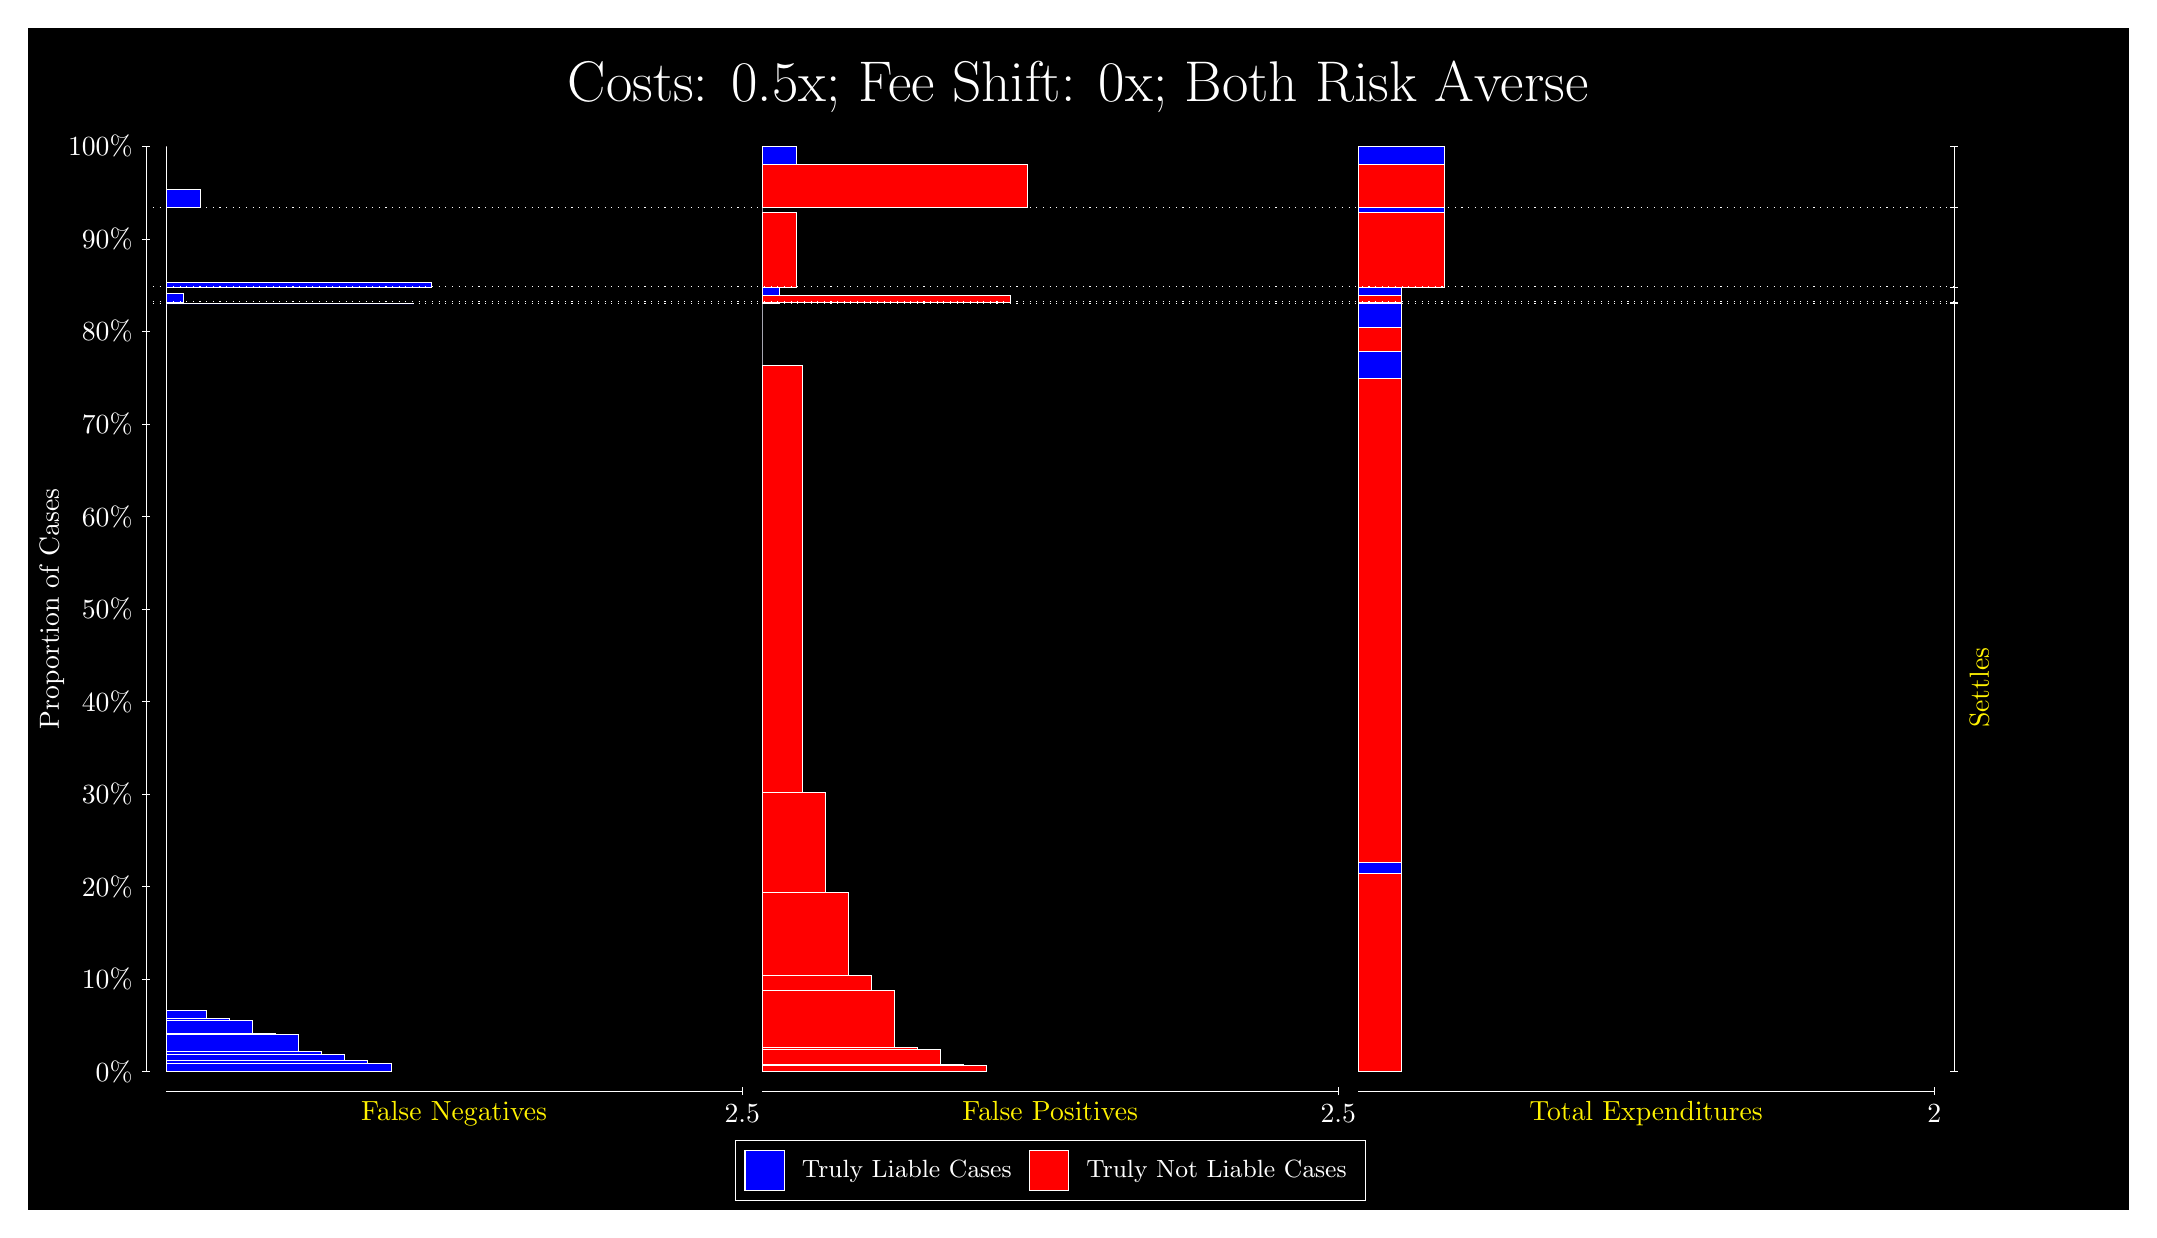
\begin{tikzpicture}
\draw[fill=black] (0,0) rectangle (26.667,15);
\draw[text=white] (0,13.5) rectangle (26.667,15) node[midway] {\huge Costs: 0.5x; Fee Shift: 0x; Both Risk Averse};
\draw[white, very thin] (1.5,1.75) -- (1.5,13.5);
\node[rotate=90, text=white, anchor=center] at (0.3, 7.625) {Proportion of Cases};
\draw[white, very thin] (1.45,1.75) -- (1.55,1.75);
\node[text=white, anchor=east] at (1.45, 1.75) {0\%};
\draw[white, very thin] (1.45,2.925) -- (1.55,2.925);
\node[text=white, anchor=east] at (1.45, 2.925) {10\%};
\draw[white, very thin] (1.45,4.1) -- (1.55,4.1);
\node[text=white, anchor=east] at (1.45, 4.1) {20\%};
\draw[white, very thin] (1.45,5.275) -- (1.55,5.275);
\node[text=white, anchor=east] at (1.45, 5.275) {30\%};
\draw[white, very thin] (1.45,6.45) -- (1.55,6.45);
\node[text=white, anchor=east] at (1.45, 6.45) {40\%};
\draw[white, very thin] (1.45,7.625) -- (1.55,7.625);
\node[text=white, anchor=east] at (1.45, 7.625) {50\%};
\draw[white, very thin] (1.45,8.8) -- (1.55,8.8);
\node[text=white, anchor=east] at (1.45, 8.8) {60\%};
\draw[white, very thin] (1.45,9.975) -- (1.55,9.975);
\node[text=white, anchor=east] at (1.45, 9.975) {70\%};
\draw[white, very thin] (1.45,11.15) -- (1.55,11.15);
\node[text=white, anchor=east] at (1.45, 11.15) {80\%};
\draw[white, very thin] (1.45,12.325) -- (1.55,12.325);
\node[text=white, anchor=east] at (1.45, 12.325) {90\%};
\draw[white, very thin] (1.45,13.5) -- (1.55,13.5);
\node[text=white, anchor=east] at (1.45, 13.5) {100\%};

\draw[white, very thin] (24.457,1.75) -- (24.457,13.5);
\draw[white, very thin] (24.407,1.75) -- (24.507,1.75);
\node[anchor=west] at (24.407, 1.75) {};
\draw[white, very thin] (24.407,11.501) -- (24.507,11.501);
\node[anchor=west] at (24.407, 11.501) {};
\draw[white, very thin] (24.407,11.524) -- (24.507,11.524);
\node[anchor=west] at (24.407, 11.524) {};
\draw[white, very thin] (24.407,11.715) -- (24.507,11.715);
\node[anchor=west] at (24.407, 11.715) {};
\draw[white, very thin] (24.407,12.727) -- (24.507,12.727);
\node[anchor=west] at (24.407, 12.727) {};
\draw[white, very thin] (24.407,13.5) -- (24.507,13.5);
\node[anchor=west] at (24.407, 13.5) {};

\draw[white, very thin, fill=blue] (1.75,1.75) rectangle (4.6044,1.8596);
\draw[white, very thin, fill=blue] (1.75,1.8596) rectangle (4.3116,1.8944);
\draw[white, very thin, fill=blue] (1.75,1.8944) rectangle (4.0188,1.9719);
\draw[white, very thin, fill=blue] (1.75,1.9719) rectangle (3.7261,2.003);
\draw[white, very thin, fill=blue] (1.75,2.003) rectangle (3.4333,2.2274);
\draw[white, very thin, fill=blue] (1.75,2.2274) rectangle (3.1406,2.241);
\draw[white, very thin, fill=blue] (1.75,2.241) rectangle (2.8478,2.4062);
\draw[white, very thin, fill=blue] (1.75,2.4062) rectangle (2.5551,2.4215);
\draw[white, very thin, fill=blue] (1.75,2.4215) rectangle (2.2623,2.5275);
\draw[white, very thin, fill=red] (1.75,2.5275) rectangle (1.75,11.501);
\draw[white, very thin, fill=blue] (1.75,11.501) rectangle (4.8971,11.501);
\draw[white, very thin, fill=red] (1.75,11.501) rectangle (1.75,11.524);
\draw[white, very thin, fill=blue] (1.75,11.524) rectangle (1.9696,11.631);
\draw[white, very thin, fill=red] (1.75,11.631) rectangle (1.75,11.715);
\draw[white, very thin, fill=blue] (1.75,11.715) rectangle (5.1167,11.774);
\draw[white, very thin, fill=red] (1.75,11.774) rectangle (1.75,12.727);
\draw[white, very thin, fill=blue] (1.75,12.727) rectangle (2.1891,12.957);
\draw[white, very thin, fill=red] (1.75,12.957) rectangle (1.75,13.5);
\draw[white, very thin, fill=red] (9.3189,1.75) rectangle (12.173,1.8284);
\draw[white, very thin, fill=red] (9.3189,1.8284) rectangle (11.88,1.8433);
\draw[white, very thin, fill=red] (9.3189,1.8433) rectangle (11.588,2.0324);
\draw[white, very thin, fill=red] (9.3189,2.0324) rectangle (11.295,2.0581);
\draw[white, very thin, fill=red] (9.3189,2.0581) rectangle (11.002,2.7797);
\draw[white, very thin, fill=red] (9.3189,2.7797) rectangle (10.709,2.9718);
\draw[white, very thin, fill=red] (9.3189,2.9718) rectangle (10.417,4.0239);
\draw[white, very thin, fill=red] (9.3189,4.0239) rectangle (10.124,5.2921);
\draw[white, very thin, fill=red] (9.3189,5.2921) rectangle (9.8312,10.723);
\draw[white, very thin, fill=blue] (9.3189,10.723) rectangle (9.3189,11.501);
\draw[white, very thin, fill=red] (9.3189,11.501) rectangle (9.5384,11.523);
\draw[white, very thin, fill=blue] (9.3189,11.523) rectangle (9.3189,11.524);
\draw[white, very thin, fill=red] (9.3189,11.524) rectangle (12.466,11.607);
\draw[white, very thin, fill=blue] (9.3189,11.607) rectangle (9.5384,11.715);
\draw[white, very thin, fill=red] (9.3189,11.715) rectangle (9.758,12.668);
\draw[white, very thin, fill=blue] (9.3189,12.668) rectangle (9.3189,12.727);
\draw[white, very thin, fill=red] (9.3189,12.727) rectangle (12.686,13.27);
\draw[white, very thin, fill=blue] (9.3189,13.27) rectangle (9.758,13.5);
\draw[white, very thin, fill=red] (16.888,1.75) rectangle (17.437,4.2625);
\draw[white, very thin, fill=blue] (16.888,4.2625) rectangle (17.437,4.4058);
\draw[white, very thin, fill=red] (16.888,4.4058) rectangle (17.437,10.558);
\draw[white, very thin, fill=blue] (16.888,10.558) rectangle (17.437,10.892);
\draw[white, very thin, fill=red] (16.888,10.892) rectangle (17.437,11.201);
\draw[white, very thin, fill=blue] (16.888,11.201) rectangle (17.437,11.501);
\draw[white, very thin, fill=red] (16.888,11.501) rectangle (17.437,11.523);
\draw[white, very thin, fill=blue] (16.888,11.523) rectangle (17.437,11.524);
\draw[white, very thin, fill=red] (16.888,11.524) rectangle (17.437,11.607);
\draw[white, very thin, fill=blue] (16.888,11.607) rectangle (17.437,11.715);
\draw[white, very thin, fill=red] (16.888,11.715) rectangle (17.986,12.668);
\draw[white, very thin, fill=blue] (16.888,12.668) rectangle (17.986,12.727);
\draw[white, very thin, fill=red] (16.888,12.727) rectangle (17.986,13.27);
\draw[white, very thin, fill=blue] (16.888,13.27) rectangle (17.986,13.5);
\draw[white, dotted] (1.5,11.501) -- (24.457,11.501);
\draw[white, dotted] (1.5,11.524) -- (24.457,11.524);
\draw[white, dotted] (1.5,11.715) -- (24.457,11.715);
\draw[white, dotted] (1.5,12.727) -- (24.457,12.727);
\draw[white, very thin] (1.75,1.5) -- (9.0689,1.5);
\node[text=yellow, anchor=north] at (5.4094, 1.5) {False Negatives};
\draw[white, very thin] (9.0689,1.45) -- (9.0689,1.55);
\node[text=white, anchor=north] at (9.0689, 1.45) {2.5};

\draw[white, very thin] (9.3189,1.5) -- (16.638,1.5);
\node[text=yellow, anchor=north] at (12.978, 1.5) {False Positives};
\draw[white, very thin] (16.638,1.45) -- (16.638,1.55);
\node[text=white, anchor=north] at (16.638, 1.45) {2.5};

\draw[white, very thin] (16.888,1.5) -- (24.207,1.5);
\node[text=yellow, anchor=north] at (20.547, 1.5) {Total Expenditures};
\draw[white, very thin] (24.207,1.45) -- (24.207,1.55);
\node[text=white, anchor=north] at (24.207, 1.45) {2};

\node[text=yellow, centered, rotate=90] at (24.777, 6.6253) {Settles};





\draw (12.978300999999998,1.5) node[draw=none] (baseCoordinate) {};
\begin{scope}[align=center]
        \matrix[scale=0.5, draw=white, below=0.5cm of baseCoordinate, nodes={draw}, column sep=0.1cm]{
            \node[rectangle, draw, minimum width=0.5cm, minimum height=0.5cm, fill=blue] {}; &
            \node[draw=none, font=\small, text=white] (B) {Truly Liable Cases}; &
            \node[rectangle, draw, minimum width=0.5cm, minimum height=0.5cm, fill=red] {}; &
            \node[draw=none, font=\small, text=white] (B) {Truly Not Liable Cases}; \\
            };
\end{scope}

\end{tikzpicture}
\end{document}